The analysis results are interpreted in terms of limits on the effective Planck
scale in $4 + n$ dimensions $\md$ in terms of the \gls{add}
model~\cite{ADDPaper} for \gls{led}. To this end a binned likelihood fit that
includes both the signal and background predictions to all the exclusive
$\met > 400$~GeV (see \cref{sec:fit-strategy}) regions EM4--EM10 as defined in
\cref{sec:event-selection-1} is performed.

\cref{fig:kfactors} reports the V + jets and the top processes normalization
factors obtained from the background only fit and applied to the \gls{mc}
predictions. It can be seen that a multiplicative factor of $1.35 \pm 0.13$ and
$0.87 \pm 0.23$ is calculated for the V + jets and top background respectively.
\begin{figure}[!h]
  \centering
  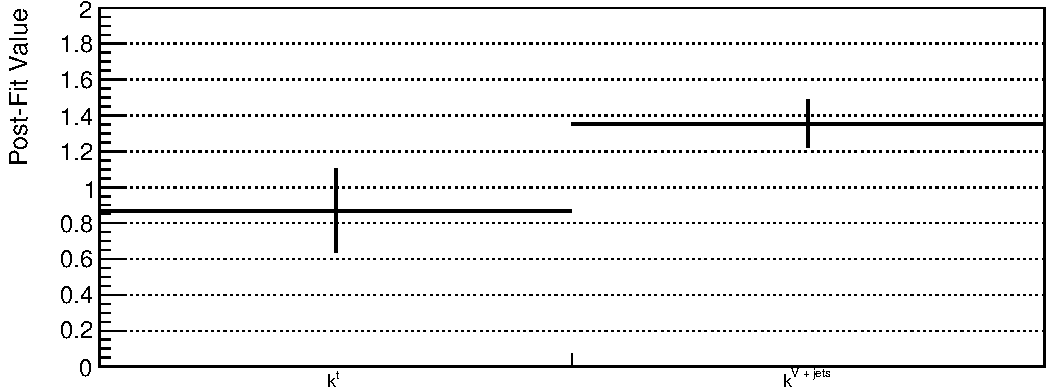
\includegraphics[width=\linewidth]{kfactors}
  \caption{Values of the normalization factors for the V + jets and single top
    backgrounds after the background only fit to the data that includes both the
    control and signal regions in all the exclusive $\met$ bins EM1-EM10 defined
    in the analysis.}
  \label{fig:kfactors}
\end{figure}

The nuisance parameters defined in \cref{sec:syst-uncert-1} and used to estimate
the impact of the systematic uncertainties on the background predictions are
treated as bin-wise correlated and treated accordingly in the
fit. \cref{fig:np_pull} shows the value of the nuisance parameters after the
background only fit to the data of the control and signal regions. In most cases
there is a mild constrain of the parameters.
\begin{figure}[!h]
  \centering
  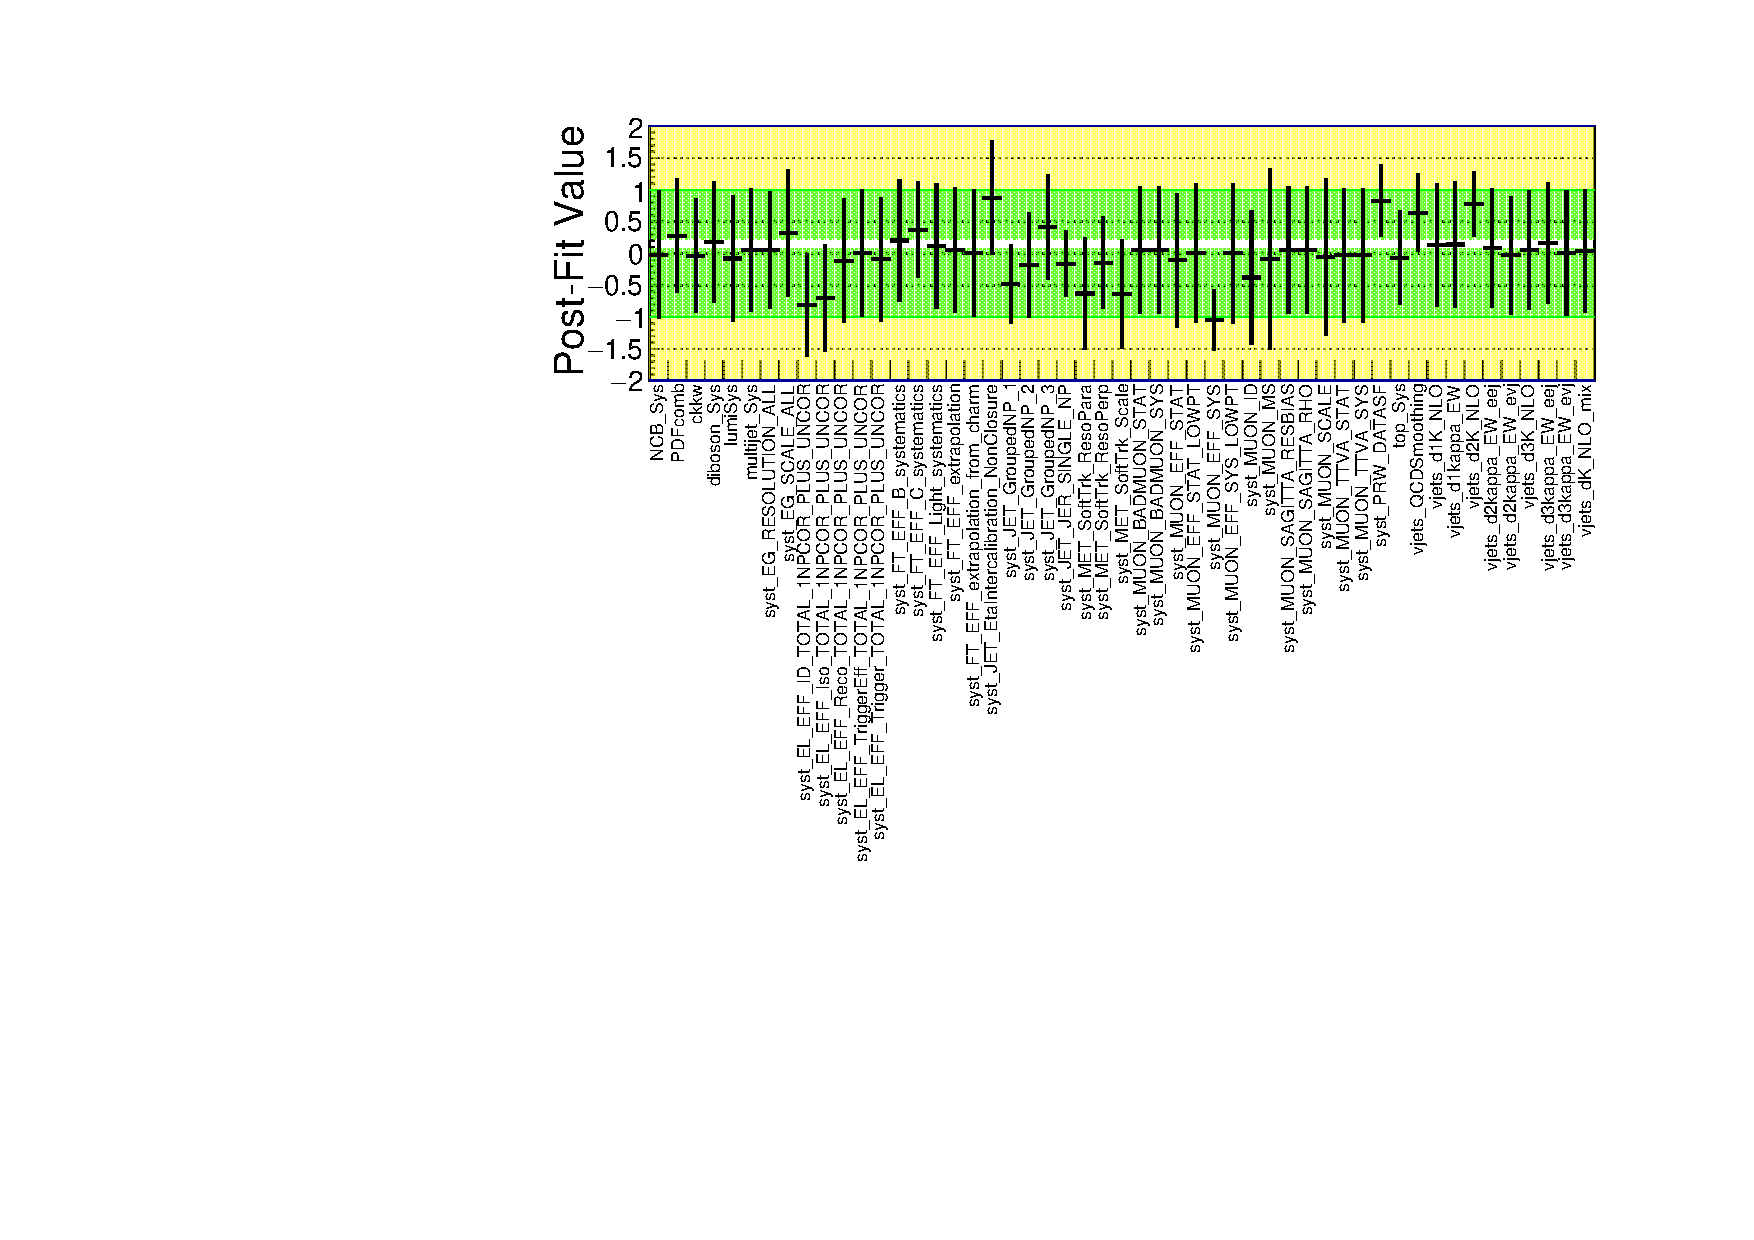
\includegraphics[width=\linewidth]{np_pull_plot}
  \caption{Values of the nuisance parameters used in the analysis after the
    control and signal region inclusive fit to the data.}
  \label{fig:np_pull}
\end{figure}

\cref{tab:add_fit_yields} reports the number of observed and predicted events in
some of the exclusive control regions defined in the analysis and used in the
background only fit to the signal and control regions.
\begin{table}[!h]
\centering
\resizebox{\linewidth}{!}{\begin{tabular}{lccccc}
\toprule
\multicolumn{6}{c}{Analysis Results} \\
\midrule \midrule
\textbf{Exclusive Signal Region } & EM4 & EM5 & EM6 & EM8 & EM9 \\
Observed events (36.1~$\ifb$) & 27843 & 8583 & 2975 & 512 & 223 \\
\midrule
SM prediction & $27893 \pm 155$ & $8542 \pm 56$ & $2935 \pm 30$ & $488 \pm 12$ & $226 \pm 5$ \\ \cline{2-6}
$\wenuplusjets$ & $1781 \pm 44$ & $525 \pm 17$ & $151 \pm 10$ & $18 \pm 2$ & $8 \pm 1$ \\
$\wmunuplusjets$ & $2021 \pm 59$ & $548 \pm 15$ & $178 \pm 6$ & $25 \pm 7$ & $12 \pm 1$ \\
$\wtaunuplusjets$ & $4829 \pm 88$ & $1323 \pm 29$ & $409 \pm 8$ & $58 \pm 5$ & $30 \pm 1$ \\
$\zeeplusjets$ & $0.02 \pm 0.02$ & $0 \pm 0$ & $0 \pm 0$ & $0 \pm 0$ & $0 \pm 0$ \\
$\zmumuplusjets$ & $35 \pm 2$ & $8 \pm 1$ & $2 \pm 0.3$ & $0.5 \pm 0.1$ & $0.5 \pm 0.1$ \\
$\ztautauplusjets$ & $70 \pm 2$ & $17 \pm 0.7$ & $5 \pm 0.2$ & $0.4 \pm 0.1$ & $0.33 \pm 0.04$ \\
$\znunuplusjets$ & $17530 \pm 196$ & $5626 \pm 59$ & $2021 \pm 25$ & $355 \pm 8$ & $164 \pm 4$ \\
$t \bar{t}$, single top & $731 \pm 89$ & $184 \pm 23$ & $42 \pm 7$ & $5 \pm 1$ & $1.5 \pm 0.5$ \\
Diboson & $863 \pm 64$ & $301 \pm 30$ & $125 \pm 16$ & $26 \pm 5$ & $9 \pm 2$ \\
Multijet background & $13 \pm 13$ & $6 \pm 5$ & $1.3 \pm 1.2$ & $0.5 \pm 0.5$ & $0.1 \pm 0.1$ \\
Non-collision background & $17 \pm 17$ & $4 \pm 4$ & $0 \pm 0$ & $0 \pm 0$ & $0 \pm 0$ \\
\bottomrule
\end{tabular}}
\caption{Number of events in the observed data and Standard Model predictions in
  a representative set of signal regions as defined in
  \cref{sec:event-selection-1}. For the \gls{sm} predictions the quoted
  uncertainty includes both statistical and systematic uncertainties.}
\label{tab:add_fit_yields}
\end{table}

\cref{fig:add_observed} show the expected and observed limits at 95\% CL on
$\md$ as a function of the large extra dimensions $n$. The dashed blue line
shows the expected limits using $36.1~\ifb$ with the $\pm 1 \sigma$ and
$\pm 2 \sigma$ error bands (green and yellow band respectively). The previous
results obtained with $3.2~\ifb$ are also reported for comparison, as can be
seen a significant improvement to the analysis is expected. The observed limit
(solid black line) is significantly worse than the expectations but within
uncertainties. This is due to the excess of data compared to \gls{sm}
predictions as reported in \cref{tab:results}.

In \cref{tab:add_limits} the limits where a M$^4_\mathrm{\, D} / \hat{s}^2$
weighting factor (see \cref{sec:valid-effect-field}) is applied to the visible
cross section for events with $\hat{s} > $ M$^2_\mathrm{\, D}$ (soft damping)
where $\hat{s}$ is the center of mass energy squared of the interacting partons
is also reported in parentheses. The effect of the the truncation is only
noticeable in the \gls{add} n = 6 model meaning that the analysis is probing
values of $\md$ where the effective theory can be trusted.

Values of $\md$ up to 7.7~TeV for n = 2 dimensions and 4.8~TeV for n = 6
dimensions are excluded at 95\%~CL improving previous results.
\begin{table}[!hb]
  \centering
  \begin{tabular}{lcc}
    \toprule
    \multicolumn{3}{c}{95\% CL Limits on M$_\mathrm{\, D}$
    [TeV]} \\
    \midrule \midrule
    ADD Model & Expected & Observed (damped) \\
    \midrule
    n = 2 & 9.2$^{+0.8}_{-1.0}$ & 7.7$^{+0.4}_{-0.5}$ (7.7) \B \\
    n = 3 & 7.1$^{+0.5}_{-0.6}$ & 6.2$^{+0.4}_{-0.5}$ (6.2) \T \B \\
    n = 4 & 6.1$^{+0.3}_{-0.4}$ & 5.5$^{+0.3}_{-0.5}$ (5.5) \T \B \\
    n = 5 & 5.5$^{+0.3}_{-0.3}$ & 5.1$^{+0.3}_{-0.5}$ (5.1) \T \B \\
    n = 6 & 5.2$^{+0.2}_{-0.3}$ & 4.8$^{+0.3}_{-0.5}$ (4.8) \T \\
    \bottomrule
  \end{tabular}
  \caption{Expected and observed 95\% CL lower limits on the fundamental Plank
      scale M$_\mathrm{\, D}$ in $4 + n$ dimensions as a function of the number
      of extra dimensions $n$. The impact of the $\pm 1 \sigma$ uncertainty from
      the theory on the observed limits and the expected $\pm 1 \sigma$ range of
      limits in absence of a signal is reported. The 95\% CL observed limits
      after damping the signal cross section for $\hat{s} > M_D^2$ are also
      reported in parentheses.}
  \label{tab:add_limits}
\end{table}

The expected sensitivity of this search to $\md$ has increased significantly
thanks to a dataset ten times larger than the previous search and improved
techniques for background calculations in particular to constrain the top and
the V + jets backgrounds. The sensitivity is dominated by systematics xx, yy,
zz. Due to the dependence of the cross section vs MD of the form A =
B$^{1/(n+2)}$ further increase in sensitivity will be difficult without reduced
systematics and much larger datasets (of the order of at least 10 times
larger). The final limits show an improvement lesser than expected due to the
observation of somewhat higher event yields in SR than predicted, however of the
order of xxx sigma. Finally it is worth to note that the new limits are so high
that the number of ADD events where the EFT is invalid, is now negligible, while
it was still non-negliglble in the previous ATLAS ADD search [REf].
\begin{figure}
  \centering
  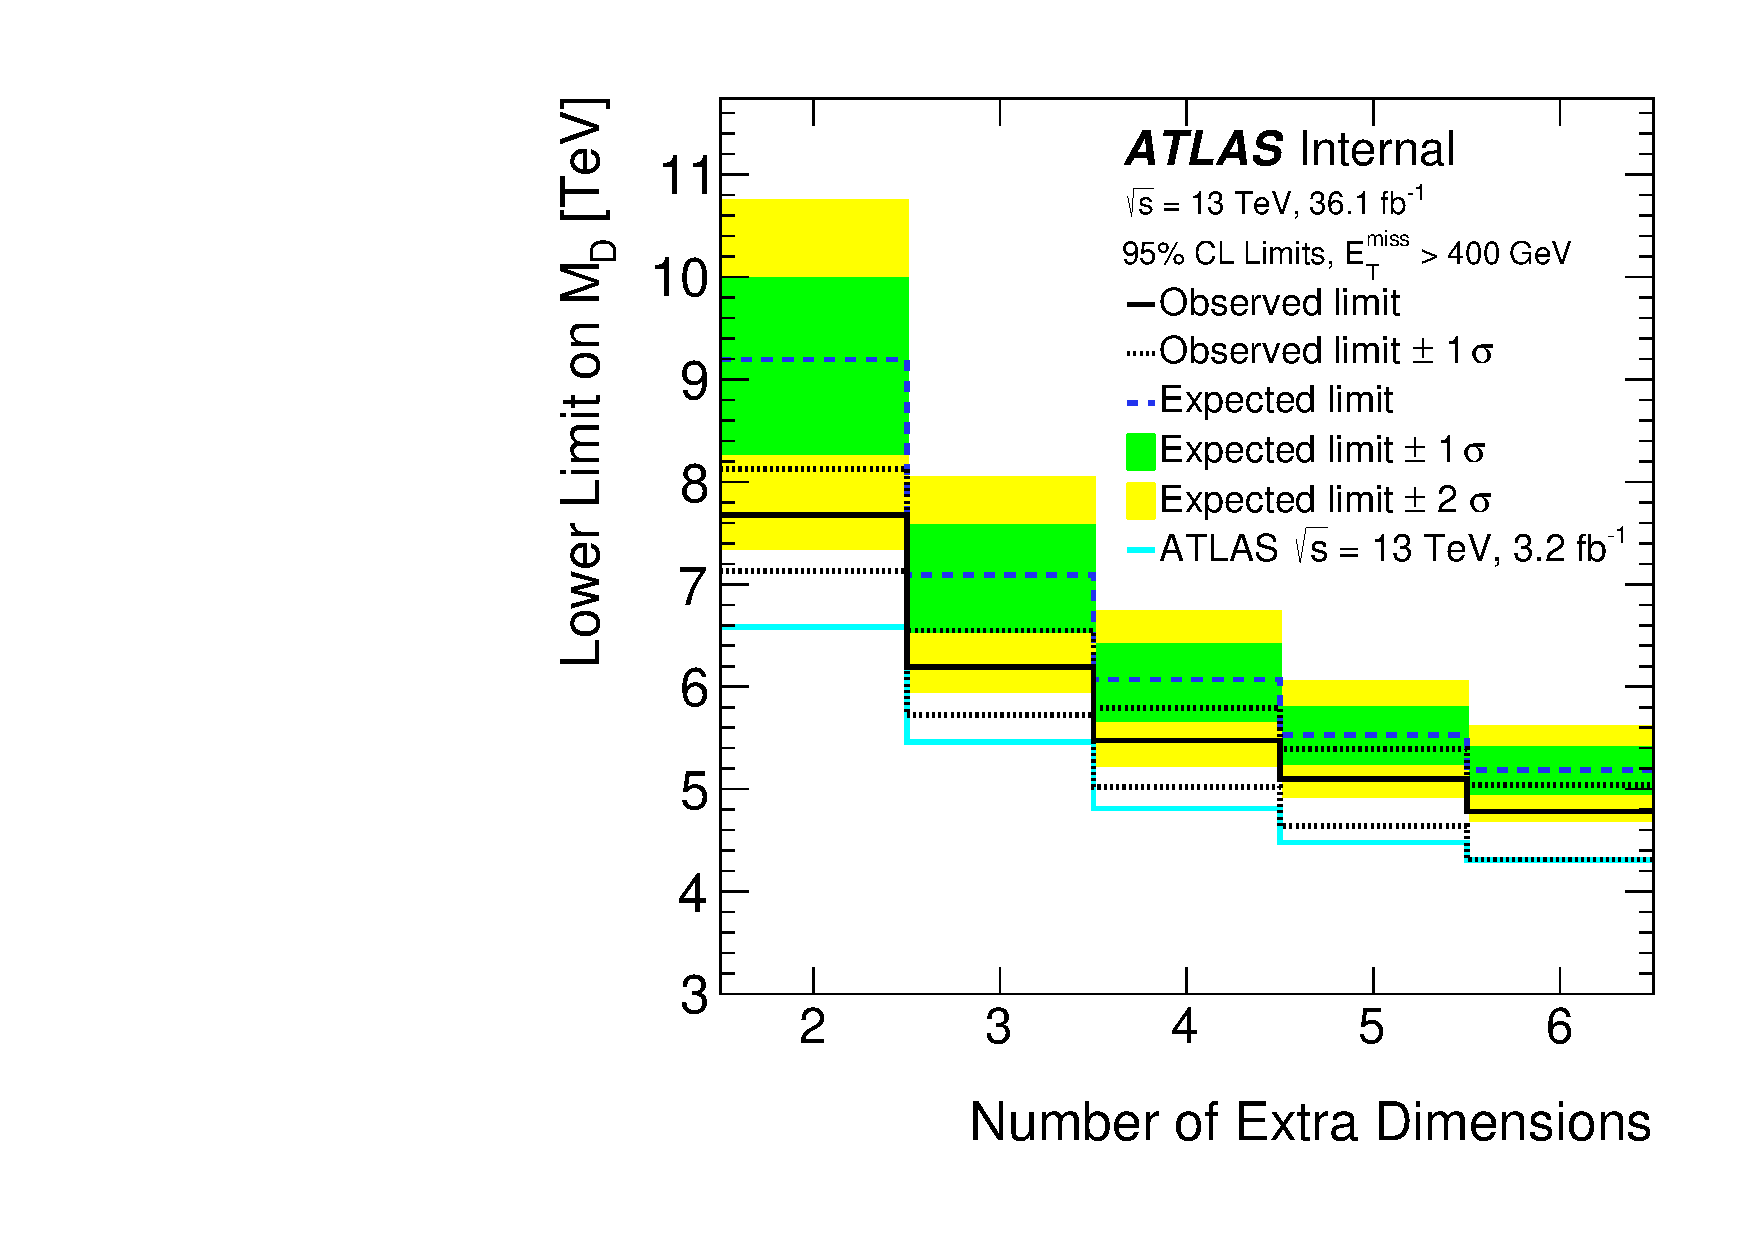
\includegraphics[width=10cm]{add_exclusion_observed}
  \caption{Expected and observed limits at 95\% CL on the fundamental Planck
    Scale in $4 + n$ dimensions, M$_\mathrm{\, D}$, as a function of the number
    of extra dimensions $n$. The dashed blue line shows the expected limit using
    $36.1~\ifb$, the green and yellow bands are the $\pm 1 \sigma$ and
    $\pm 2 \sigma$ uncertainties on the estimate. The solid black line is the
    observed limit while the cyan line represents the observed limits in the
    2015 analysis using $3.2~\ifb$.}
  \label{fig:add_observed}
\end{figure}
%%% Local Variables:
%%% mode: latex
%%% TeX-master: "../search_for_DM_LED_with_ATLAS"
%%% End:
